\documentclass[12pt, letterpaper]{article}
\usepackage{graphicx}

\title{Visualizing ocean data with OceanSpy}
\author{Sourav Barua}
\date{August 5, 2020}

\begin{document}

\maketitle

\section{Introduction}
Ocean Current Simulation using numerical circulation models have become so realistic at present. These simulation models generate a large volume of model output data, making the analysis of model data harder. Using OceanSpy, model data can be easily analyzed in the way observational oceanographers analyze field measurements.  OceanSpy\footnote{https://github.com/hainegroup/oceanspy} is an open-source and user-friendly Python package that enables scientists and interested amateurs to analyze and visualize ocean model datasets.

In this project, I use the demo data provided by OceanSpy to demonstrate their two plotting method TS\_diagram() and horizontal\_section() to create a Temperature vs. Salinity plot and a temperature with depth plot. 
 


\section{Methods}

\subsection{Dataset}
The dataset used for this demonstration is the demo date provided by OceanSpy. These data contain High-resolution (~2km) numerical simulation covering the east Greenland shelf (EGshelf), and the Iceland and Irminger Seas (IIseas) forced by the Arctic System Reanalysis (ASR). These data can be downloaded from https://livejohnshopkins-my.sharepoint.com/:u:/g/personal/
malmans2\_jh\_edu/EXjiMbANEHBZhy62oUDjzT4BtoJSW2W0tYtS2qO8\_SM5m
Q?download=1



\subsection{Marine Heat Waves}

To quantify whether SST for a particular area is indeed abnormally warm, we will use the Marine Heatwave (MHW) definition of Hobday et al. (manuscript submitted to Progress in Oceanography).  An algorithm for detecting a MHW has been implemented in the Python package `marineHeatWave`.

\begin{figure}
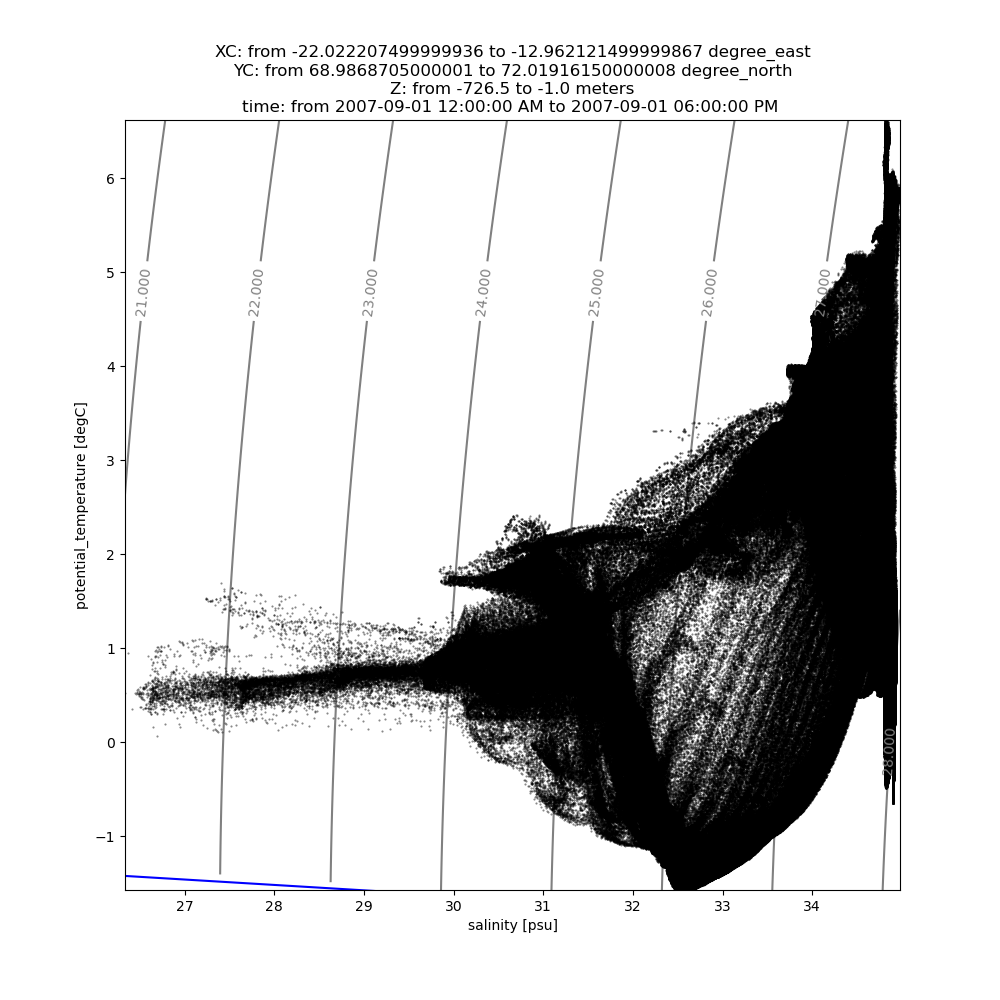
\includegraphics[width=0.9\textwidth]{TempvsSalinity}
\caption{SST over time from at Station 44225 with QC codes shown}
\label{fig:TempvsSalinity}
\end{figure}



\section{Results}

As shown in Figure~\ref{fig:TempvsSalinity}, the SST has a typical annual cycle between about $0^\circ$ C and $20^\circ$ C. There is some missing data between the years 2002 and 2004.  In 2005, 2006, and 2008 there is
increased noise in the data suggesting that something is wrong with the data.  It would be strange for the SST to be considerably below zero.  More significantly, the data from early 2010 is very suspicious as it suggests that the temperature is getting close to $80^\circ$ C.  Clearly we need to clean this dataset before continuing to analyze it.



This dataset from the Marine Environmental Data Section (MEDS) of the Department of Fisheries and Oceans (DFO) has already gone a quality control (QC) process. The results of QC are given by a numerical code as describe in Table~\ref{tbl:qc_codes}.








\section{Conclusions}


% would be good to a a bibilography here too.

\end{document}